\documentclass{article}
\usepackage{graphicx} % Required for inserting images
\usepackage{algpseudocode}
\usepackage{algorithm}
\usepackage{blindtext}
\usepackage{geometry}
 \geometry{
 a4paper,
 total={170mm,257mm},
 left=20mm,
 top=20mm,
 }



\title{Semester 1 Reduced Notes}
\author{Finlay Ross-Davie}
\date{January 2024}



\begin{document}
\maketitle

\section{Asymptotics}

\textbf{Little o}

In general, f is o(g) if $$\forall c > 0.\exists N. \forall n \geq N. f(n) < cg(n)$$

This is equivalent to saying $$\frac{g(n)}{f(n)} \rightarrow \infty \; as \; n \rightarrow \infty$$

I.e 'f is slower-growing than' or 'asymptotically smaller than g' \newline

\textbf{Little omega - $\omega$}

$\omega$ is the converse of $o$ and $f = \omega(g)$ can be read as saying: 'f is asymptotically smaller than / grows slower than g'

f = $\omega(g)$ if any only if $g = \omega(f)$ \newline

\textbf{Big O}

$f \; is \; O(g)$ can be read as 'f grows no faster than g' or f is eventually bounded above by some (sufficiently large multiple Cg of g), formally:

$$\exists C >0. \exists N. \forall n \geq N. f(n) \leq Cg(n)$$

Write as f is O(g), and call g an \textbf{asymptotic upper bound for f} \newline

\textbf{Omega - $\Omega$}

$f \; is \; \Omega (g)$ reads as 'f grows no slower than g' or g is an \textbf{asymptotic lower bound} for f 

$f=\Omega g$ says f is eventually bounded below by some multiple of cg of g: 
$$\exists c > 0. \exists N. \forall n \geq N. cg(n) \leq f(n)$$

\textbf{Big $\theta$}

$f \; is \; \theta(g)$ can be read as g is an asymptotically tight bound for f or f and g essentially have the same growth rate. 

$f \; is \; \theta g$ if both $f \in O(g) \; and \; f \in \Omega(g)$

Formally, 

$$\exists c_1, c_2 > 0. \exists N. \forall n \geq N. c_1g(n) \leq f(n) \leq c_2g(n)$$ \newline

A Big-O Complexity chart for standard growth rates is shown below

\begin{figure}[ht]
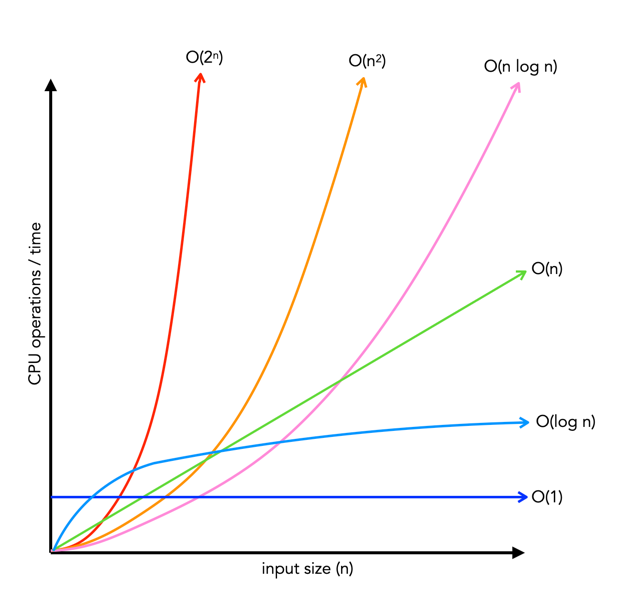
\includegraphics[width=8cm]{Big O complexity chart.png}
\centering
\end{figure}

\section{Lists, Stacks, Queues}

The time-complexities of common \textbf{Array(list)} operations are:
\begin{itemize}
    \item Add or remove an element at the end: $O(1)$
    \item Add or remove element from arbitrary index: $O(n)$
    \item Access or modify element at arbitary index: $O(1)$
    \item Check if element exists: $O(n)$
    
\end{itemize}

The time-complexities of common operations for \textbf{immutable strings} are:

\begin{itemize}
    \item Add or remove character: $O(n)$
    \item Access element at arbitrary index: $O(1)$
    \item Create substring: $O(m)$, where $m$ is the length of the substring
    \item Concatenation between two strings: $O(n+m)$, where m is the length of the other string
\end{itemize}

The time-complexities of common operations for \textbf{linked lists} are:
\begin{itemize}
    \item Add or remove element given pointer before add/removal location: $O(1)$ (single and doubly linked)
    \item Add or remove element at arbitrary position without pointer: $O(n)$
    \item Access element at arbitrary position without pointer: $O(n)$
    \item Check if element exists: $O(n)$
    \item Reverse between position i and j: $O(j-i)$
\end{itemize}

The time complexities of common operations for \textbf{stacks} are:
\begin{itemize}
    \item Push element: $O(1)$
    \item Pop element: $O(1)$
    \item Peek: $O(1)$
    \item Access or modify element at arbitrary index: $O(1)$
    \item Check if element exists: $O(n)$
\end{itemize}

The time complexities of common operations for \textbf{Queues} are
\begin{itemize}
    \item Enqueue element: $O(1)$
    \item Dequeue element: $O(1)$
    \item Peek: $O(1)$
    \item Access or modify element at arbitrary index: $O(n)$
    \item Check if element exists: $O(n)$
\end{itemize}

\section{Sets, dictionaries and hashing}

A \textbf{Set} is an unordered collection of objects/items of a given type X \\

contains: $X \rightarrow bool$ \\
insert: $X \rightarrow void$ \\
delete: $X \rightarrow void$ \\
isEmpty $void \rightarrow bool$ \\

The time complexities of common operations for \textbf{Sets} are:
\begin{itemize}
    \item Add or remove element: $O(1)$
    \item Check if element exists: $O(1)$
\end{itemize}

A \textbf{dictionary} is a general-purpose data structure for storing a group of objects. A dictionary has a set of keys and each key has a single associated value. When presented with a key, the dictionary will return the associated value. \\

Hash maps are indexed data structures. A hash map makes use of a hash function to compute an index with a ket into an array of buckers or slots. Its value is mapped to the bucket with the corresponding index. Hash function is the core of implementing a hash map. It takes the key and translates it to the index of a bucket in the bucket list \\



lookup: $X \rightarrow Y$ \\
insert: $X * Y \rightarrow void$ \\
delete: $X \rightarrow void$ \\
isEmpty: $void \rightarrow bool$ \\

The time complexities of common operations for \textbf{Hash table/dictionaries} are:
\begin{itemize}
    \item Add or remove key-value pair: $O(1)$
    \item Check if key exists: $O(1)$
    \item Check if value exists: $O(n)$
    \item Access or modify value associated with key: $O(1)$
    \item Iterate over all keys, or both: $O(n)$
\end{itemize}

The time complexities of common operations for \textbf{Heap/Priority queues } are:
\begin{itemize}
    \item Add an element: $O(logn)$
    \item Delete the minimum element: $O(logn)$
    \item Find the minimum element: $O(1)$
    \item Check if element exists: $O(n)$
\end{itemize}

\section{Standard Algorithms}

\begin{table}
    \centering

    \begin{tabular}{r|ccc}

    Algorithm & Best Case & Average Case & Worst Case\\
    \hline

    Bubble Sort & \(O(n)\) & \(O(n^2)\) & \(O(n^2)\)\\
    Insertion Sort & \(O(n)\) & \(O(n^2)\) & \(O(n^2)\)\\
    Merge Sort & \(O(nlogn)\) & \(O(nlogn)\) & \(O(nlogn)\)\\
    Heap Sort & \(O(nlogn)\) & \(O(nlogn)\) & \(O(nlogn)\)\\
    Quick Sort & \(O(nlogn)\) & \(O(nlogn)\) & \(O(n^2)\)\\


    \hline
    \end{tabular}

\end{table}




\end{document}